\chapter{Az antik Róma művészete} % Introduction
\label{ch:3_antik_roma}

\section{Az antik Róma korszakai, kultúrája, építészete, szobrászata és festészete}

\tcbox[left=0mm,right=0mm,top=0mm,bottom=0mm,boxsep=0mm,
toptitle=0.5mm,bottomtitle=0.5mm,title=\centering{A tétel adatai}]{%
	
	\begin{tabular}{| p{0.25\textwidth} | p{0.7\textwidth} |}
		\hline
		Tétel teljes címe
		& 
		Mutassa be az antik Róma korszakait, kultúráját, építészetének, szobrászatának és festészetének jellegzetésseit! Soroljon fel és jellemezzen néhány fennmaradt római építményt és alkotást!
		\\ \hline
		
		Jegyzetek &
		\begin{compactitem}
			\item Az ókori Római Birodalom társadalmi felépítése, a római művészet korszakai és jellemzői.
			\item Az építészet jellemzői, építmény-típusai, a szobrászat és festészet emlékei.
			\item Pannónia provincia római kori maradványai.
		\end{compactitem}
		\\\hline
		
	\end{tabular}}

\subsection*{Történelmi háttér}

	Róma alapításaként a Kr.e. 753-as évszámot jelöli meg a történelem. A Római Birodalom népe, a latinok mellett az etruszk és a szabin nép élt az itáliai félsziget északi részén.
	
	Kezdetben ezek közül az etruszkok voltak a legjelentősebbek. Kr.e. a VIII. sz. -ban telepedtek le a mai Toszkána területén (ma Siena, Pisa, Firenze e terület legfőbb városai). Az etruszk kultúra virágkora a Kr.e. VI.-VII.sz. volt. Az etruszkok kis városállamokat alapítottak, később Kr.e. 600 körül szövetségre léptek a környező népekkel. Így hozták létre Latium központtal, Róma fővárossal a Római Birodalom még kisméretű elődjét.
	
	A VII.sz.-tól a Kr.e. első századig terjed a királyok kora, amikor királyok uralkodnak a még Itáliánál messzebbre ki nem terjedő Római Birodalom területén.
	
	A Római Birodalom virágkora a Kr.e. első századra tehető, amikortól a császárok korát számítjuk. Ebben a periódusban nő meg igen nagy mértékben a birodalom területe: a mai Spanyol- és Franciaország, Anglia déli része, a német területek déli része, a Dunántúl, a Balkán-félsziget, a görög félsziget, Kis-Ázsia, Palesztina területe, Egyiptom és Afrika észai partvidéke tartozik hozzá.
	
	A Római Birodalom a Kr.u. V.sz.-ban ketté válik: Nyugat-Római és Kelet-Római Birodalommá. Kr.u. 476-ban a népvándorlás, az Európát elárasztó barbár népek betöréseinek következtében a Nyugat-Római Birodalom megbukik, míg a keleti rész Bizánc néven fejlődésnek indul.

\subsection*{Társadalom}

A király feladatait (hadvezér, bíró és főpap) az előkelők osztották fel maguk között. Óvintézkedésként az egyeduralom újbóli kialakulása ellen a vezető tisztségviselőket, így a consulokat is csak egy évre, és kettesével választották, hogy egymást is ellenőrizhessék. A kialakult szisztéma számos eleme a római köztársaság korát is túlélte.

A társadalom vertikális szerkezete viszonylag egyszerű volt, mivel legalábbis kezdetben csupán az előkelőkből és a tőlük függő helyzetben levő népből állt. Az alacsonyabb származású személyeknek és családoknak az egyes előkelőkhöz való rendkívül szoros kötődése, a cliensi viszony vagy klientúra különböző formákban Róma egész történelme folyamán fennmaradt.

\subsection*{Hitvilág}

Az ókori Róma fennállása alatt sok vallási kultusz befolyása alatt állt, melyekből sokat átvett. A római istenségekkel a római mitológia foglalkozik.

A túlvilágról a rómaiaknak mindvégig homályos elképzeléseik voltak, mindenesetre az ősök szellemeit mélyen tisztelték, igyekeztek kiengesztelni őket. A házi oltárokon, melyeknek papja a családfő volt, naponta áldoztak kisebb ajándékokkal, étellel, gyümölccsel, kevés borral vagy olajjal.

\tcbox[left=0mm,right=0mm,top=0mm,bottom=0mm,boxsep=0mm,
toptitle=0.5mm,bottomtitle=0.5mm,title=\centering{Római istenek}]{%
	\begin{tabular}{| p{0.25\textwidth} | p{0.25\textwidth} | p{0.45\textwidth} |}
		\hline
		\textbf{Római istenek }
		&
		\textbf{Görög istenek}
		&
		\textbf{Meghatározás}
		\\ \hline\hline
		
		Zeusz & Jupiter & a legfőbb isten
		\\ \hline
		
		Poszeidon & Neptunus & a tengerek istene
		\\ \hline
		
		Hádész & Pluto & az alvilág istene
		\\ \hline
		
		Niké & Victoria 	& a győzelem istennője
		\\ \hline
		
		Árész & Mars & a háború istene
		\\ \hline
		
		Apollón & Apollo & a jóslás és költészet istene
		\\ \hline
		
		Hesztia & Vesta & a házi tűzhely istennője
		\\ \hline
		
		Artemisz & Diana & a vadászat, a hold istennője
		\\ \hline
		
		Héra & Juno & a házastársi hűség istennője
		\\ \hline
		
		Themisz & Justitia & az igazság istennője
		\\ \hline
		
		Aphrodité & Venus & a szépség, a szerelem istennője
		\\ \hline
\end{tabular}}

\begin{center}
	\tcbox[colback=darkgray!85!black,
	left=0mm,right=0mm,top=0mm,bottom=0mm,boxsep=1mm,toptitle=0.5mm,bottomtitle=0.5mm,
	title=\centering{A római panteon második fő istentriásza: Jupiter a főhelyen, Juno és Minerva}]{
		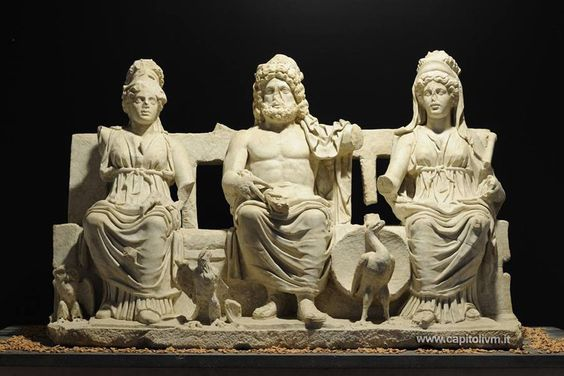
\includegraphics[width=0.7\linewidth]{03/romai_istenek}}
\end{center}

\subsection*{Építészet}

Tiszteli a görög kultúrát, így tovább viszi a görög építészet vívmányait, díszítő és tagoló elemeit. Funkcionális, célszerűségre törekszik, logikus, jól érthető.


\subsubsection{Új építészeti találmányok}

\paragraph{Cementfalazás}
A rómaiak új falazási módot alakítanak ki, új anyagokat alkalmaznak, ez a cementfalazás. Sajátossága, hogy a kívül lévő héjszerű kő és téglarakás között, belül egy cementes kőtörmelékből falmag található. Előnye: erősebb, tartósabb, mint az egyszerű kőrakás, valamint íves felületeket könnyebben lehet kialakítani vele.

\paragraph{Boltíves-pilléres szerkezet}
A rómaiak egy forradalmian új szerkezetet, tartórendszert alakítanak ki: a boltíves-pilléres szerkezetet. A görögök az oszlopos-gerendázatos szerkezetet alkalmazták, ahol az oszlop hordta a súlyt, és a vízszintes gerenda fedte le, hidalta át a teret. A boltíves-pilléres szerkezet előnye a gerendázattal szemben az, hogy több súlyt bír el, és nagyobb távolságot is át tud ívelni, hidalni. Ha a gerendás oszlopos szerkezetnél a súlyt vagy a fesztávolságot növelték, a gerenda egyszerűen eltört, mivel a súly a gerenda közepére nehezedett! A boltíves szerkezetnél az íven a súly eloszlik, és megosztva nehézkedik a pillérekre.

\paragraph{Térlefedési módok}
cementfalazással és a boltíves-pilléres szerkezettel olyan új térlefedési módokra nyílt lehetőség, amelyek íves falat képeznek, és a boltívhez hasonlóan vezetik le a súlyt. Ezek a dongaboltozat, a keresztboltozat és a kupola.
\begin{compactitem}
	\item Dongaboltozat: félhenger formájú boltozat.
	\item Keresztboltozat: két dongaboltozat kereszteződése négyzet alaprajzon.
	\item Kupola: félgömb formájú boltozat (kör alaprajzú tér fölött).
\end{compactitem}

\begin{figure}[H]
	\centering
	\tcbox[colback=darkgray!85!black,
	left=0mm,right=0mm,top=0mm,bottom=0mm,boxsep=1mm,toptitle=0.5mm,bottomtitle=0.5mm,
	title=\centering{Dongaboltozat és keresztboltozat}]{
		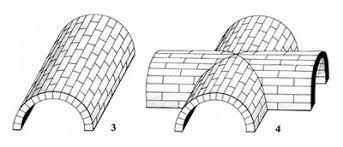
\includegraphics[width=0.7\linewidth]{03/terlefedes_1}}
	\captionsetup{labelformat=empty}
	\caption{}
\end{figure}

\begin{wrapfigure}{r}{0.35\textwidth}
	\tcbox[colback=darkgray!85!black,
	left=0mm,right=0mm,top=0mm,bottom=0mm,boxsep=1mm,toptitle=0.5mm,bottomtitle=0.5mm,
	title=\centering{Kompozit oszlopfejezet}]{
		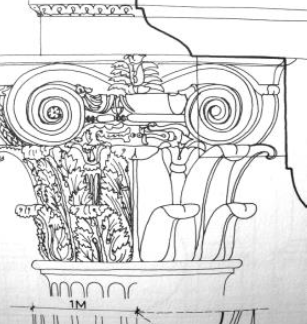
\includegraphics[width=1.0\linewidth]{03/kompozit_oszlopfejezet}
	}
\end{wrapfigure}

\paragraph{Kompozit oszlopfejezet}
A rómaiak tovább használják a görög oszloprendeket, de gyakran ún. oszlopszékre (henger vagy hasáb formájú talapzat) helyezik az oszlopokat.
A görög oszloptípusok mellett kialakul egy negyedik oszlopfejezet is: a kompozit oszlopfő, ami a ión csigavonal (voluta) és a korintoszi akantuszlevél motívumait ötvözi, arányait tekintve a görög korintoszi oszlophoz hasonló.

\clearpage

\subsubsection{A mérnöki építészet}

\begin{wrapfigure}{r}{0.45\textwidth}
	\tcbox[colback=darkgray!85!black,
	left=0mm,right=0mm,top=0mm,bottom=0mm,boxsep=1mm,toptitle=0.5mm,bottomtitle=0.5mm,
	title=\centering{Pons Mulvius híd}]{
		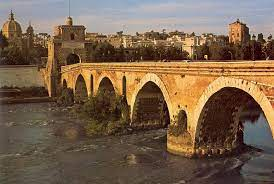
\includegraphics[width=1.0\linewidth]{03/pons_mivius_hid}
	}
	\tcbox[colback=darkgray!85!black,
	left=0mm,right=0mm,top=0mm,bottom=0mm,boxsep=1mm,toptitle=0.5mm,bottomtitle=0.5mm,
	title=\centering{Vízvezeték}]{
	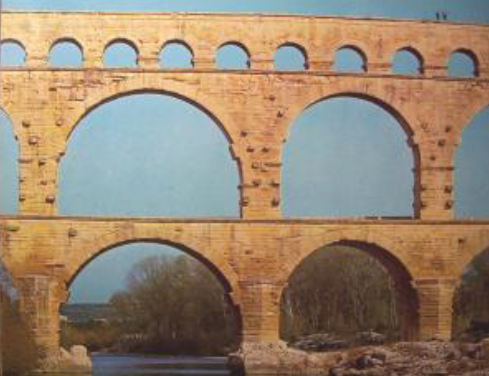
\includegraphics[width=1.0\linewidth]{03/vizvezetek}
	}
\end{wrapfigure}

\paragraph{Utak}
A rómaiak Európa-szerte hatalmas, jól kiépített úthálózatot alakítanak ki, ami a kor infrastruktúráját jelentette.

\paragraph{Hidak}
A boltíves-pilléres szerkezettel az első nagyméretű hidakat a rómaiak építik. A leghíresebb máig álló római kori híd: Pons Mulvius Rómában.

\paragraph{Vízvezetékek}
Nagyméretű, több kilométeres hosszúságú, több szintes, boltíves-pilléres szerkezetű építmény, aminek segítségével a hegyvidékből a természetes lejtést kihasználva a városokba szállították a vizet.

\paragraph{Városépítészet}
Két várostípus volt alaprajz és kialakítás alapján.

	\subparagraph{Kolónia}
	A rómaiak által meghódított városok az ún. kolóniák: a szabálytalan alakú városfalat megerősítik, és a város úthálózatát négyzetrácsossá alakítják.
	
	\subparagraph{Castrum}
	A rómaiak által alapított városok a római katonai tábornok ( ún. „castrum”) mintájára épültek: nem csak úthálózatuk szabályos, hanem a városfalak is szabályos, derékszögű négyzet vagy téglalap alakúak. Ilyen pl: Ostia (Róma közelében található)

\paragraph{Fórum}
A római fórum a római város hosszanti elrendezésű, téglalap jellegű \textbf{főtere}, ahol oszlopcsarnokok, és templom áll. A fórum kereskedelmi, politikai célokat szolgált.

	\begin{wrapfigure}{r}{0.35\textwidth}
		\tcbox[colback=darkgray!85!black,
		left=0mm,right=0mm,top=0mm,bottom=0mm,boxsep=1mm,toptitle=0.5mm,bottomtitle=0.5mm,
		title=\centering{Forum Romanum}]{
			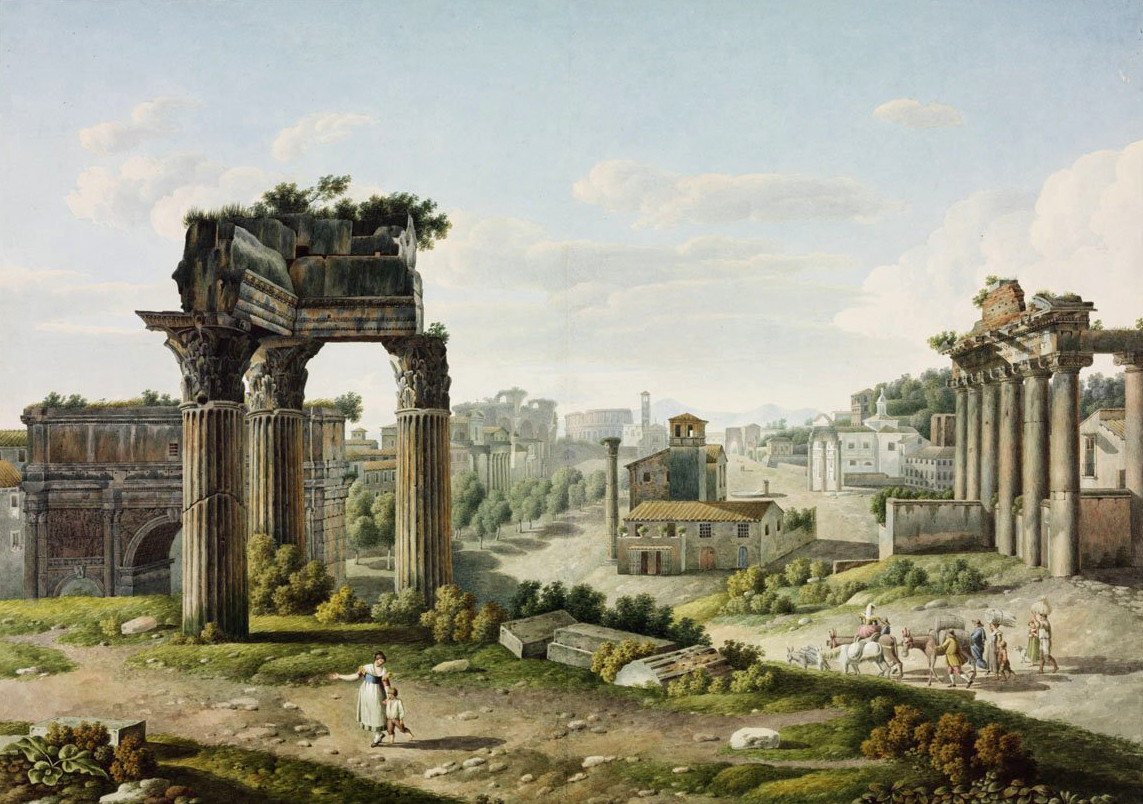
\includegraphics[width=1.0\linewidth]{03/forum_romanum}
		}
	\end{wrapfigure}

	\subparagraph{Forum Romanum} Rómában található, Róma leghíresebb műemlékei közé tartozik. Sokáig piactér volt, majd elkezdték bővíteni, több évszázadig, több királyi és császári dinasztia alatt gyarapodott (mindegyik császár épített hozzá valamit), ezért alakja newm követi a szabályos fórum-sémát. Körülbelül 150m hosszú terület, számos templom, politikai épület (többek közt a római szenátus gyűlésterme), diadalívek találhatók rajta.

\begin{wrapfigure}{r}{0.25\textwidth}
	\tcbox[colback=darkgray!85!black,
	left=0mm,right=0mm,top=0mm,bottom=0mm,boxsep=1mm,toptitle=0.5mm,bottomtitle=0.5mm,
	title=\centering{Diadalív}]{
		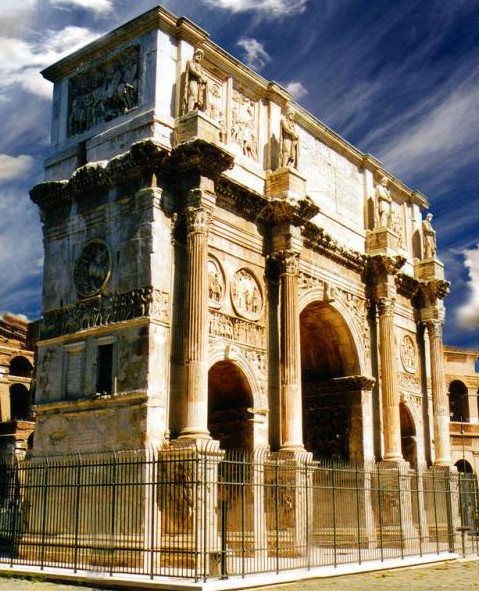
\includegraphics[width=1.0\linewidth]{03/diadaliv.jpeg}
	}
\end{wrapfigure}

\paragraph{Diadalív}
Egy vagy három kapuból álló építmény, ami eredetileg arra szolgált, hogy a diadalmenetek során megtisztítsa a győztes csatából hazatérő római katonákat a háború bűneitől. Később a meghódított területeken felállítva a Római Birodalom győzelmét és hatalmát hirdették. A diadalív felületén általában a győztes csatát vagy a felvonulást ábrázoló domborművek találhatók.

\paragraph{A római bazilika}
fórum két hosszanti oldalán található \textbf{nem vallásos} rendeltetésű középület, ami gazdasági, politikai, társadalmi célokat szolgált, piac, bíráskodás helye lehetett.
Alaprajza: hosszanti elrendezésű, az épület bejárata a fórum felől, azaz a hosszabbik oldalon nyílik

\subparagraph{Belső tere} A belsőbe állított oszlopsorok segítségével több hajó (= osztatlan belső tér) alakul ki, így a belső tágas, célja, hogy minél nagyobb számú tömeget legyen képes befogadni

\subparagraph{Szerkezete} A fő és mellékhajót oszlopsorok választják el egymástól. A mellékhajó falán nincsenek ablakok, az épület megvilágítását a főhajó kiemelkedő falán lévő ablakok szolgáltatták, itt jött be a fény. Ezt a szerkezeti felépítést bazilikális szerkezetnek nevezzük.

\paragraph{Termák}
Más néven fürdők. A rómaiak által kedvelt közösségi helyeknek egyike. A görögöktől vették át. Általában 3 medencéjük volt: hideg vizes, langyos, melegvizes, amik az íves kőboltozatokkal voltak lefedve: donga-, keresztboltozattal és kupolával. A melegvizű medencéket és a fürdő többi helyiségét a padlóban és a falakban futó agyagcsövek segítségével melegítették.

\paragraph{Teátrumok és Amfiteátrumok}

	\subparagraph{Teátrum}
	Görög színház, amit a rómaiak átvettek azzal a különbséggel, hogy nem sziklába vájták a színházat, a nézőtér súlyát nem a hegyoldal tartotta meg, hanem ők maguk építették fel az alépítményt is az íves boltozatok felhasználásával. A római teátrum is félkör alakú, mint a görög.
	
	\subparagraph{Amfiteátrum}
	Kör alakú teátrum, ilyen például a Colosseum (Róma).	

\paragraph{Colosseum}

	\subparagraph{Története}
	Eredeti neve Amfiteátrum Flávium volt, mert a Flavius császári dinasztia ideje alatt épült Kr.u. 70-80 között. Az építkezést Titus császár fejezte be. Az épület a nevét a mellette álló hatalmas, kolosszális méretű Néró császárt ábrázoló szoborról kapta. Mivel az amfiteátrum Flávium a Római Birodalom legnagyobb amfiteátruma volt (50 ezer néző befogadására volt alkalmas) méltán magáévá tette a méreteire utaló Colosseum nevet.
	
	\tcbox[colback=darkgray!85!black,
	left=0mm,right=0mm,top=0mm,bottom=0mm,boxsep=1mm,toptitle=0.5mm,bottomtitle=0.5mm,
	title=\centering{A Colosseum ma és régen}]{
		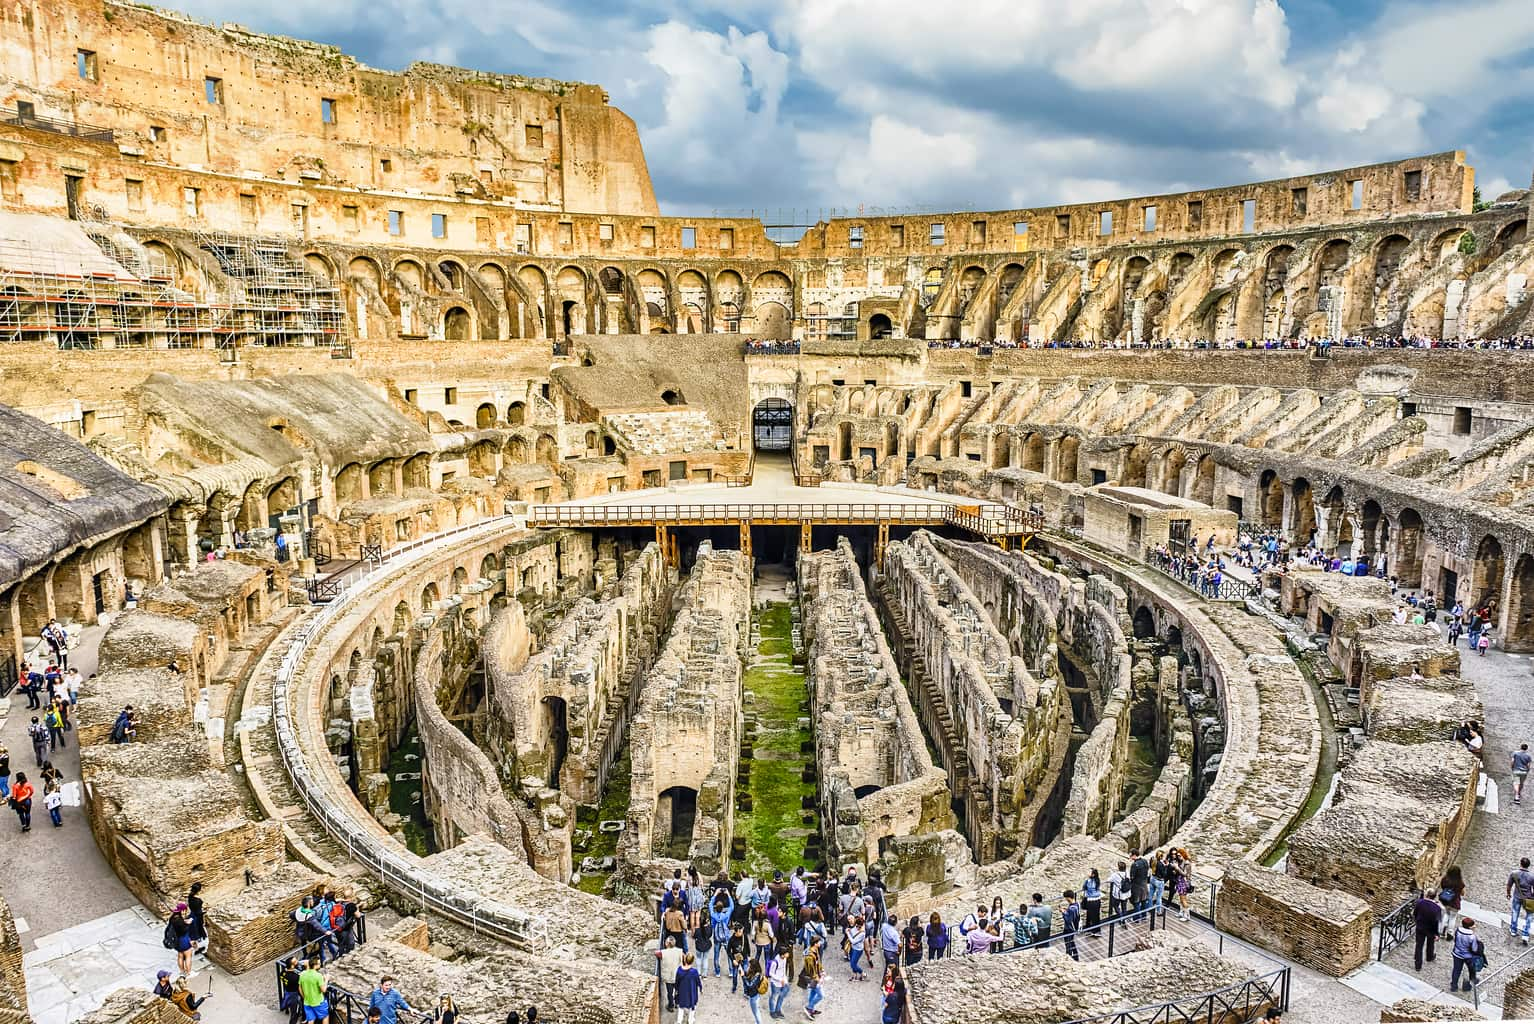
\includegraphics[width=0.49\linewidth]{03/colosseum}
		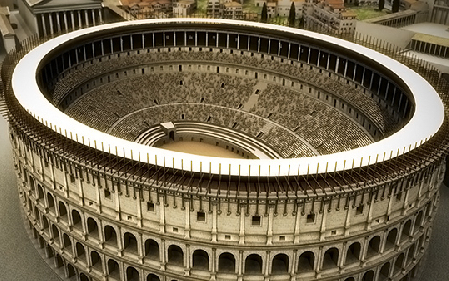
\includegraphics[width=0.49\linewidth]{03/colosseum_rekonstrukcio}
	}
	
	\subparagraph{Rendeltetés}
	Az épületben gladiátor játékok és állatviadalok zajlottak. A római császárok gyakran a győztes római hadjáratokat játszatták el a gladiátorokkal. A Colosseum padlóját szigetelni lehetett, így akár vízi csaták bemutatására is volt lehetőség.
	
	\subparagraph{Alaprajz}
	A Colosseum ellipszis alaprajzú, belső része az aréna (a Róma közelében lévő tengerpart arany színű homokjáról kapta a nevét, ezzel szórták be), a játékok helye, amit körben alépítménnyel megtámasztott nézőtér övez.
	
	\subparagraph{Szerkezet és térlefedés}
	A nézőteret íves boltozatok támasztják alá, vezetik le a súlyát. A nézőtérre a sugár irányú és körbefutó folyosókon keresztül lehetett bejutni, amelyek számára a boltozatok lefedést biztosítanak. Főleg dongaboltozattal fedték ezeket a folyosókat.
	
	\subparagraph{Homlokzat}
	Három szinten árkádok (boltív + pillér) sorolódnak egymás mellé, az e fölötti szint áttörés, nyílás nélküli fal, elsősorban az árnyékolást biztosította. Az árkádok között féloszlopok kaptak helyet: alul dór, középen ión, felül korintoszi, legfelül kompozit oszlopok. Noha az oszlopok nem vesznek részt a súly alátámasztásában, az oszloprendek sorrendje a teher levezetésének megfelelően alakult, a legnagyobb teherbíró képességgel rendelkező oszloptípust került legalulra, és az egyre kisebb terhet viselni tudok egyre feljebb. A római építészetnek az az elve nyilvánul meg ebben, hogy még a díszítőelem kialakítása is a logikát tükrözi. Ezt a homlokzati kialakítást Colosseum-motívumnak nevezzük.

\subsubsection{Templomépítészet}

A római templomépítészetben megnyilvánul a görög kultúra szeretete: a római templomok követik görög elődeiket, azokból alakulnak ki.

\paragraph{Különbségek a görög templomoktól}
\begin{compactitem}
	\item Nem magaslatra épülnek, hanem síkságra, a városba, a fórum rövidebb oldalára. Ezért a görög templomokkal ellentétben a római templomoknál kialakul a főhomlokzat: azaz elsősorban egy, a fórum felé néző homlokzatukkal érvényesülnek, az oldalsó és hátsó homlokzataik kevésbé hangsúlyosak.
	
	\item Nem veszi körbe minden oldalról lépcsős talapzat, hanem csak a főhomlokzatra vezet fel lépcső, a többi rész egy pódiumon áll.
	
	\item Főhomlokzatuk arányai a széles görög templomokkal ellentétben keskenyebbek és magasabbak.
\end{compactitem}

\paragraph{Két típusa}

	\subparagraph{Álperipterosz}
	Hosszanti elrendezésű templomtípus a görög peripterosz alaprajzból alakul ki, de míg a görög peripteroszt minden oldalról oszlopok veszik körül, a római épület oldal- és hátsó homlokzatán az oszlopok nem szabadon állnak, hanem féloszlopokká alakulnak, azaz a falhoz tapadnak.
	
	\subparagraph{Tholosz}
	Az azonos nevű, kerek, oszlopokkal körülvett görög templomtípust követi
	Vesta templom: tholosz alaprajzú templom, Korintoszi oszlopok veszik körül a falát. A vesta szüzek temploma volt. Sajátossága, hogy nincs gerendázata. A görög tholosz alaprajztól az különbözteti meg, hogy a római templomokhoz méltón pódiumon áll.

\begin{figure}[H]
	\centering
	\begin{minipage}{0.6\textwidth}
		\tcbox[colback=darkgray!85!black,
		left=0mm,right=0mm,top=0mm,bottom=0mm,boxsep=1mm,toptitle=0.5mm,bottomtitle=0.5mm,
		title=\centering{Álperipterosz}]{
			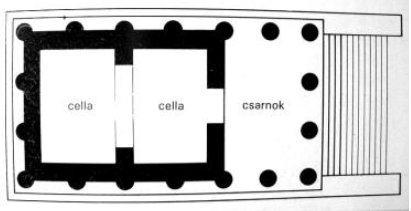
\includegraphics[width=1.0\linewidth]{03/alperipterosz}
		}
	\end{minipage}
	\hfill
	\begin{minipage}{0.35\textwidth}
		\tcbox[colback=darkgray!85!black,
		left=0mm,right=0mm,top=0mm,bottom=0mm,boxsep=1mm,toptitle=0.5mm,bottomtitle=0.5mm,
		title=\centering{Vesta templom, Róma}]{
			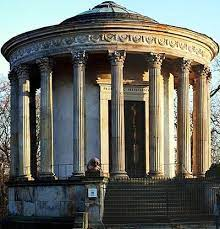
\includegraphics[width=1.0\linewidth]{03/vesta_templom}
		}
	\end{minipage}
\end{figure}

\paragraph{Pantheon}

	\subparagraph{Történet}
	A Pantheont a római építészet csúcsának is tartják. Kr.u. 120-130-ig épült. A Pantheon név (pan = összes, theosz = isten) az összes római istenre utal, akiknek szentelték a templomot. Az épületnek nem csak a neve, homlokzata is hasonlít az athéni Parthenónhoz: oszlopos timpanonos, de oszlopfejezetei korintosziak.
	
	\subparagraph{Alaprajz}
	2 részből áll: egy téglalap alakú előcsarnokból, melyet oszlopok több részre osztanak és egy hatalmas osztatlan kör alakú térből. Ez a belső 43 m átmérőjű volt, és térlefedésének másfél évezredig csodájára jártak, mert egészen a reneszánszig nem tudtak hasonlót építeni.

\begin{center}
	\tcbox[colback=darkgray!85!black,
	left=0mm,right=0mm,top=0mm,bottom=0mm,boxsep=1mm,toptitle=0.5mm,bottomtitle=0.5mm,
	title=\centering{Pantheon, Róma}]{
		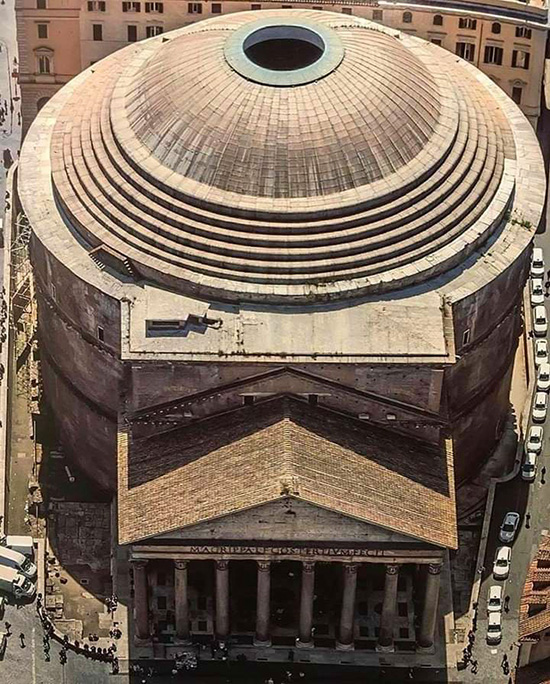
\includegraphics[width=0.45\linewidth]{03/pantheon}
		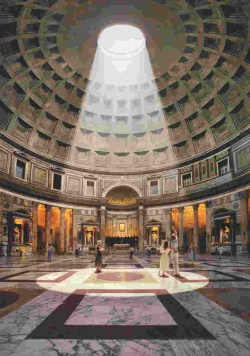
\includegraphics[width=0.4\linewidth]{03/pantheon_belseje}
	}
\end{center}

	
	\subparagraph{Térlefedés}
	A 43 m átmérőjű osztatlan belső tér egyetlen kupolával van lefedve.
	
	\subparagraph{Szerkezet}
	Ahhoz, hogy ekkora súlyt meg tudjanak tartani a falak, a következőkre volt szükség:
	\begin{compactitem}
		\item rendkívül erős falak: 6-7 m széles falvastagság
		\item ne bontsa meg semmilyen nyílás a kupolát és a falakat: nincsenek ablakok a falakon
		\item a kupolában egymásra nehézkedő boltívek váza tartja alapvetően a súlyt
		\item amennyire csak lehet, csökkenteni kellett a kupola súlyát: ezt úgy érték el, hogy alulról fölfelé egyre kevesebb fajsúlyú köveket helyeztek, és legfelül már habkövek vannak.
	\end{compactitem}

	\subparagraph{Belső}
	A belsőben a fényt a kupola tetején lévő 9 m átmérőjű kör alakú nyílás, az opeion biztosítja, ez az épület egyetlen fényforrása. A nyíláson keresztül máig beesik a csapadék. Az épület márványburkolatos padlójában azonban kis vízelvezető tölcsérek, rések találhatók, amik hamar szárazzá teszik a felületet. A kupola belső felülete kazettás díszítésű, ami nem pusztán díszít, de szintén szerepet játszik a súlylevezetésben is. A fal középső részén timpanonos álablakok találhatók, alul szintén timpanonos keretezésű fülkék, melyekben egykor a római istenek szobrai álltak.

\subsubsection{Pompeii városa}

\begin{wrapfigure}{r}{0.45\textwidth}
	\tcbox[colback=darkgray!85!black,
	left=0mm,right=0mm,top=0mm,bottom=0mm,boxsep=1mm,toptitle=0.5mm,bottomtitle=0.5mm,
	title=\centering{Pompeii}]{
		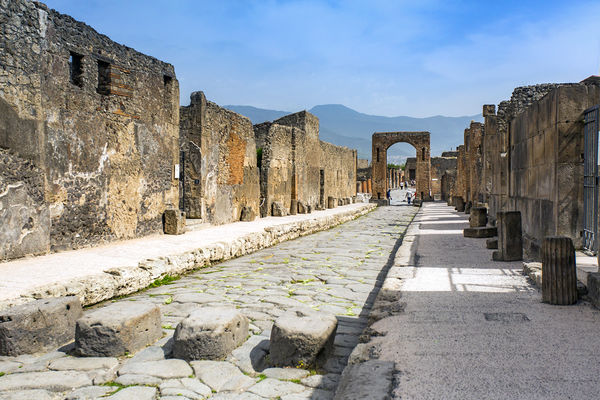
\includegraphics[width=1.0\linewidth]{03/pompeii}
	}
	\tcbox[colback=darkgray!85!black,
	left=0mm,right=0mm,top=0mm,bottom=0mm,boxsep=1mm,toptitle=0.5mm,bottomtitle=0.5mm,
	title=\centering{Pompeii lakosai}]{
		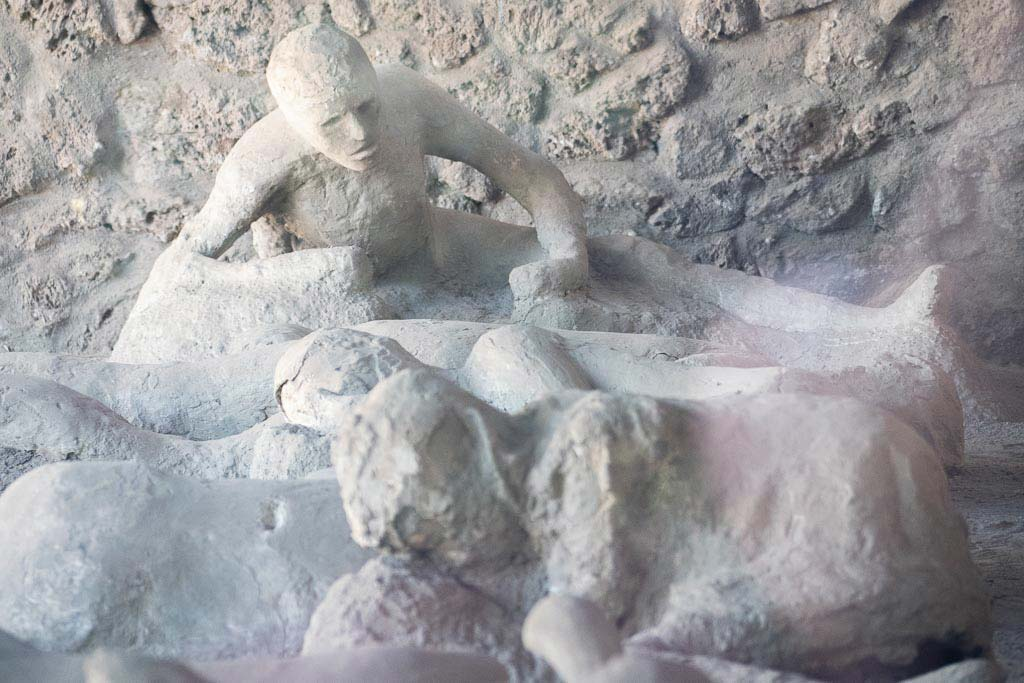
\includegraphics[width=1.0\linewidth]{03/pompeii_lakosai}
	}
\end{wrapfigure}

Rómától délre Nápoly közelében található a város, a Vezúv (vulkán) lábánál. Kr.u. 79-ben a vulkán kitört és a várost betemette a hamu és a vulkanikus kőtörmelék, így az szinte teljesen a föld alá került, és fennmaradt. (Mellette szintén hasonlóan maradt fenn Herculáneum városa, de ez kevésbé feltárt).

Pompeii vesztét az okozta, hogy a láva közvetlenül nem fenyegette, a város lakói azonban nem számítottak arra, hogy a szél a város fölé fújja a vulkanikus gázokat. A lakókat a gázok és a levegő keveredéséből keletkezett kőtörmelék és hamu fedte be kb. 3 méter magasságban. Az emberek nem tudtak elmenekülni, és a kén és széndioxid miatt megfulladtak. Herculáneumot valóban a láva pusztította el.

Pompeii bortermeléssel és textiliparral foglalkozott. A városiak valószínűleg tudtak a veszélyről, mivel a Vezúv már 10 évvel korábban is kitört egyszer, de maradtak, mert a vulkáni talaj tökéletes bortermelő vidékké tette a környéket. Fennmaradtak textiltisztító kádak, a pékség malmai, a diadalív, a főút, 3 m magasságig a lakóépületek, freskóval festett politikai hirdetések, a színház épülete, amfiteátrum, a város fóruma és bazilikái.

\clearpage

\subsection*{A Római Birodalom szobrászata}

\subsubsection{Álltalános jellemzők}

Általában valamilyen kapcsolatban áll a politikai propagandával, célja, hogy a Római Birodalom tekintélyét, méltóságát hirdesse, növelje.

Stílusbeli újításokat, újszerűségeket alig tapasztalunk:
\begin{compactitem}
	\item A római szobrászat stílusa a görög szobrászat stílusát követi (a klasszikus és hellenizmus korit). ()Ennek oka: a hellenizmus kori görög szobrászat stílusa már Nagy Sándor korában elterjedt a mai Görögország, Kis-Ázsia és Dél-Itália területén, majd a római katonák szó szerint magukkal vitték a meghódított területetek görög istenszobrait Itáliába, hogy a diadalmenetek alkalmával felmutassák azokat a győzelem jeleként. Számos másolat készül görög szobrokról. A hellenizmus kori szobrokat általában csak római másolataikból ismerjük.)
	\item A római szobrászat sajátossága a domborművészetben, hogy a közeli figurákat magasan faragják (a fejek elválnak a faltól, és ezért mára le is törtek általában), a háttér motívumainak távlatát viszont lapos faragásmóddal érzékeltetik.
	\item A domborművészet jellemzője még a folyamatos komponálás: a történet eseményei között nincsen elválasztás, a történetet balról jobbra haladva szinte olvasni lehet, tehát elbeszélő jellegű lesz.
	\item Az épületek ábrázolása, a tér a perspektíva szabályai szerint alakul.
	\item A portrészobrászatban a realizmus érvényesül.
\end{compactitem}

A római szobrászat leggyakoribb témája az allegória = valamilyen fogalom, földrajzi hely, természeti jelenség, érzelem vizuális, képi megjelenítése általában emberi alak formájában.

A római szobrászat három fő emlékcsoportja:
\begin{compactitem}
	\item Domborművek – oltárok, diadalívek, diadaloszlopok domborművei.
	\item Portré – császárok mell- és fejszobrai.
	\item Egész alakos szobrok.
\end{compactitem}


\subsubsection{Domborművek}

	\paragraph{Augusztusz oltára}
	Augustus császár, akinek politikai jelszava a béke volt, állítatta az oltárt Pax Augustának, a béke istennőjének.
	
	A szabadban felállított, kis pódiumon álló, három oldalán falakkal körülvett oltár, melynek falain domborművek vannak:
	\begin{compactitem}
		\item Az Anyaföld (Itália) allegóriája – dombormű. Gyermekeit tápláló anyaként jelenik meg Itália földje, a két keblei felé forduló gyermek az ölében Romulusra és Rémusra, tágabban a római népre utal. Körülöttük a termékeny föld adományai: állatok, növények.
		
		\item Aeneász Itáliáért áldoz- dombormű. Az előtér alakjai magasan faragottak, a háttér motívuma – a templom – lapos faragású. A lapos faragásmóddal a templom vonásai elmosódottabbnak tűnnek.
	\end{compactitem}

\begin{figure}[H]
	\begin{minipage}{0.32\textwidth}
		\tcbox[colback=darkgray!85!black,
		left=0mm,right=0mm,top=0mm,bottom=0mm,boxsep=1mm,toptitle=0.5mm,bottomtitle=0.5mm,
		title=\centering{Augusztus oltára}]{
			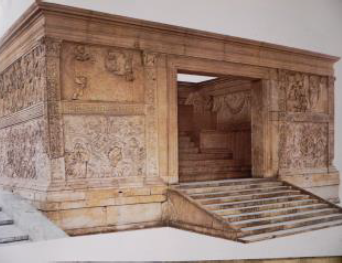
\includegraphics[width=1.0\linewidth]{03/augusztus_oltar}
		}
	\end{minipage}
	\hfill
	\begin{minipage}{0.29\textwidth}
		\tcbox[colback=darkgray!85!black,
		left=0mm,right=0mm,top=0mm,bottom=0mm,boxsep=1mm,toptitle=0.5mm,bottomtitle=0.5mm,
		title=\centering{Az Anyaföld (Itália) allegóriája}]{
			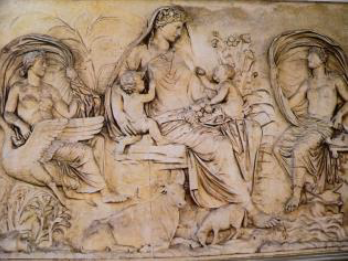
\includegraphics[width=1.0\linewidth]{03/italia_dombormu}
		}	
	\end{minipage}
	\hfill
	\begin{minipage}{0.32\textwidth}
		\tcbox[colback=darkgray!85!black,
		left=0mm,right=0mm,top=0mm,bottom=0mm,boxsep=1mm,toptitle=0.5mm,bottomtitle=0.5mm,
		title=\centering{Aeneász Itáliáért áldoz}]{
			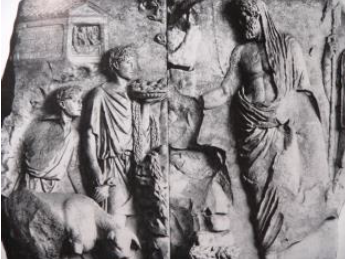
\includegraphics[width=1.0\linewidth]{03/aeneasz}
		}
	\end{minipage}		
\end{figure}
	

\paragraph{Titus diadalívének domborműve}
A jeruzsálemi hadjáratból hazatérő, a diadalmeneten felvonuló, a salamoni templom kegytárgyait bemutató (pl. menóra = hátágú gyertyatartó) katonákat ábrázolja, amint a diadalív felé haladnak. Az előtér alakjainak feje elválik a faltól – le is tört – a háttér figurái viszont laposan faragottak. A diadalív perspektivikusan ábrázolt.

\paragraph{Traianus diadaloszlopa}
Emlékműként álló oszlop, ami Traianusz császár dáciai hadjáratának állít emléket. Rajta spirálisan kb. 1 m magas, kiterítve 120 m hosszú domborműszalag meséli el a hadjáratot anélkül, hogy egyetlen kerettel megszakítaná az elbeszélés folyamatát. A jeleneteket csak a csoportszervezés különíti el egymástól némileg.

\begin{figure}[H]
	\begin{minipage}{0.5\textwidth}
		\tcbox[colback=darkgray!85!black,
		left=0mm,right=0mm,top=0mm,bottom=0mm,boxsep=1mm,toptitle=0.5mm,bottomtitle=0.5mm,
		title=\centering{Titus diadalívének domborműve}]{
			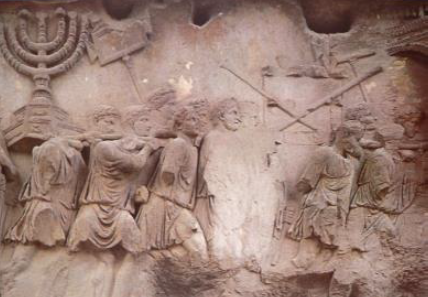
\includegraphics[width=1.0\linewidth]{03/titus_diadaliv}
		}
	\end{minipage}
	\hfill
	\begin{minipage}{0.45\textwidth}
		\tcbox[colback=darkgray!85!black,
		left=0mm,right=0mm,top=0mm,bottom=0mm,boxsep=1mm,toptitle=0.5mm,bottomtitle=0.5mm,
		title=\centering{Traianus diadaloszlopa}]{
			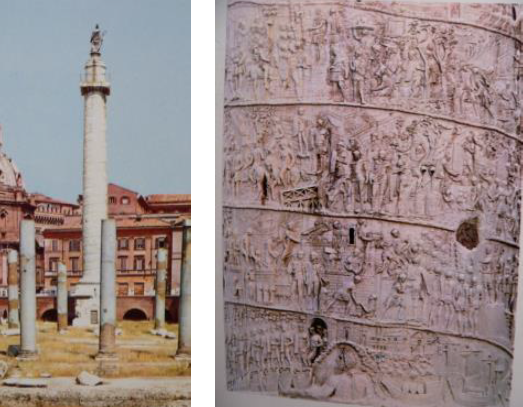
\includegraphics[width=1.0\linewidth]{03/traianus_diadaloszlopa}
		}	
	\end{minipage}	
\end{figure}

\subsubsection{Császárportrék}

\begin{wrapfigure}{r}{0.4\textwidth}
	\tcbox[colback=darkgray!85!black,
	left=0mm,right=0mm,top=0mm,bottom=0mm,boxsep=1mm,toptitle=0.5mm,bottomtitle=0.5mm,
	title=\centering{Császárportré}]{
		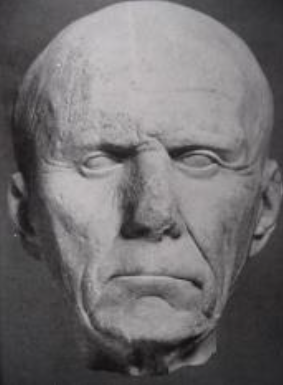
\includegraphics[width=1.0\linewidth]{03/csaszarportre}
	}
\end{wrapfigure}

	Alapvetően realizmus jellemzi a portrékat: a császárok valós vonásait tükrözik a szobrok.
	
	Néhány általános jellemző mégis mindegyiken megfigyelhető.
	
	Nem a fiatal, a görög és korábbi kultúráknál megszokott fiatal férfi jelenti az ideált, hanem az idősebb, tapasztal férfi válik eszményképpé.
	
	Erőteljes pofacsont, erősen kiugró szemöldökcsont, összeráncolt szemöldök, erős homlok és mosolyráncok, mélyen, sötét árnyékban ülő szemek, keskeny széles, összeszorított száj jellemzi a fejeket. Az arcok szigort, tekintélyt, bölcsességet, hatalmat tükröznek.

\subsubsection{Egész alakos figurák}

	\paragraph{Augusztusz egész alakos álló szobra}
	A szobor sok tekintetben követi a görög hagyományokat.
	A kontraposzt tartás és az izmos, részletesen kidogozott felsőtest a klasszikus kori szobrászat hatását mutatja (ilyen a Dárdavivő), a gazdagon, sűrűn redőző, dekoratív drapéria a hellenizmus hatására utal. (A római művészet kedveli és továbbviszi a görög hagyományokat.) A római szobrászat sajátosságai:
	Ezeket az arc kialakításában (szigorú, tekintélyt sugárzó arc) és a mellvéden található allegorikus figurákban találhatjuk meg.
	
	
	\paragraph{Marcus Aurélius lovasszobra}
	A műfaj: a bornz lovas szobor a római császárok kedvelt műfaja volt, ebben a császárok diadalmas hadvezérként lovon ülve ábrázoltatták magukat. Marcus Aurélius szobrán kívül azonban nem maradt fenn több példány. E szobor is annak köszönhette fennmaradását, hogy a középkorban azt hitték, hogy a szobor Nagy Konstantint, a kereszténységet államvallássá tévő császárt ábrázolja.
	
	\begin{figure}[H]
		\begin{minipage}{0.45\textwidth}
			\tcbox[colback=darkgray!85!black,
			left=0mm,right=0mm,top=0mm,bottom=0mm,boxsep=1mm,toptitle=0.5mm,bottomtitle=0.5mm,
			title=\centering{Augusztusz szobra}]{
				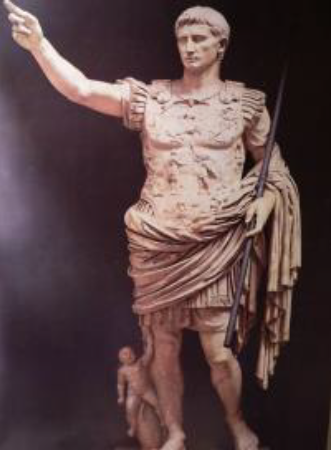
\includegraphics[width=1.0\linewidth]{03/augusztusz}
			}
		\end{minipage}
		\hfill
		\begin{minipage}{0.45\textwidth}
			\tcbox[colback=darkgray!85!black,
			left=0mm,right=0mm,top=0mm,bottom=0mm,boxsep=1mm,toptitle=0.5mm,bottomtitle=0.5mm,
			title=\centering{Marcus Aurelius lovasszobra}]{
				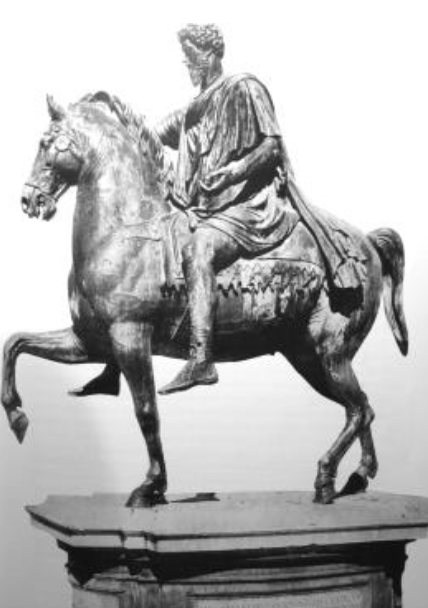
\includegraphics[width=1.0\linewidth]{03/marcus}
			}	
		\end{minipage}	
	\end{figure}

\subsection*{Az ókori Róma festészete}

A legtöbb festmény Pompeiiben maradt fenn, és a portré, a tájkép, a csendélet, a látszat-architektúra (építészeti tagozatok plasztikus, reális megfestése, imitálása) és a mitologikus témájú műfajokban készült.

\paragraph{Stílus} A realizmus, a fény-árnyékkal való modellálás, a plasztikusság jellemzi a képeket. A tájképeknél a reális térhatást a levegőperspektíva (a háttérben lévő motívumok egyre halványodnak, szürkés-kék színűekké válnak), a fény és a sötét, árnyékos felületek erős kontrasztja fokozza.

\paragraph{Technika} Falra kerülnek, leggyakrabban freskó, valamint mozaik.

	\subparagraph{Freskó technika} 
	Nedves vakolatra kerül a festék, és a vakolat mésztartalma a száradás során kiválva a falfelületen mészpáncélt hoz létre, így a freskó rendkívül tartós. Hátránya, hogy egy nap alatt kb. egy négyzetméternyi területet lehet megfesteni vele, amibe később már nem lehetett belenyúlni, nem lehet változtatni rajta.
	
	\subparagraph{Mozaik technika} A falra vagy a padlóra készül, apró kövek, festett kerámiák, színes üvegdarabokból kirakott kép.
	
\vspace{1cm}	

\tcbox[colback=darkgray!85!black,
left=0mm,right=0mm,top=0mm,bottom=0mm,boxsep=1mm,toptitle=0.5mm,bottomtitle=0.5mm,
title=\centering{Pompeii-i festmények}]{
	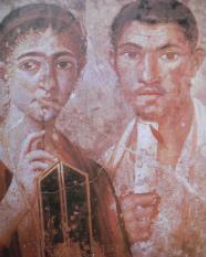
\includegraphics[width=0.34\linewidth]{03/romai_festeszet_1}
	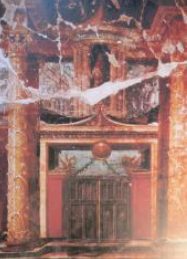
\includegraphics[width=0.31\linewidth]{03/romai_festeszet_2}
	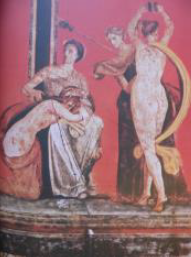
\includegraphics[width=0.33\linewidth]{03/romai_festeszet_3}
}

\clearpage

\subsection*{Pannónia provincia római kori maradványai}

\begin{wrapfigure}{r}{0.45\textwidth}
	\tcbox[colback=darkgray!85!black,
	left=0mm,right=0mm,top=0mm,bottom=0mm,boxsep=1mm,toptitle=0.5mm,bottomtitle=0.5mm,
	title=\centering{Pannonia}]{
		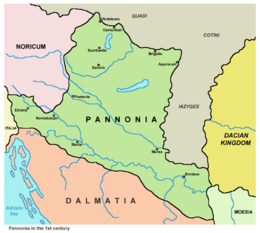
\includegraphics[width=1.0\linewidth]{03/pannonia}
	}
\end{wrapfigure}

Pannonia a Római Birodalom egyik provinciája volt. 

A rómaiak Pannonia provincia (és így a mai Magyarország területét) a Kr.u. 1. században hódították meg, több lépcsőben. A fejlődő kereskedelem miatt ekkor lett fontos ez a provincia. Kr.e.14-ig a Balatontól nyugatra lévő területeket foglalták el a római seregek (itt húzodott a Borostyánút), majd fokozatosan a Duna vonaláig haladtak. (Pannonia magában foglalja Kelet-Ausztriát, Szlovákia Dévény-Pozsony környéki részét, Észak-Szlovéniát, a Dunántúlt, Észak-Horvátországot, Észak-Szerbia egy részét és Bosznia-Hercegovina északi sávját is.) A mai Magyarország területén számtalan római település maradványait tárták fel.

\begin{wrapfigure}{r}{0.45\textwidth}
	\tcbox[colback=darkgray!85!black,
	left=0mm,right=0mm,top=0mm,bottom=0mm,boxsep=1mm,toptitle=0.5mm,bottomtitle=0.5mm,
	title=\centering{Aquincum}]{
		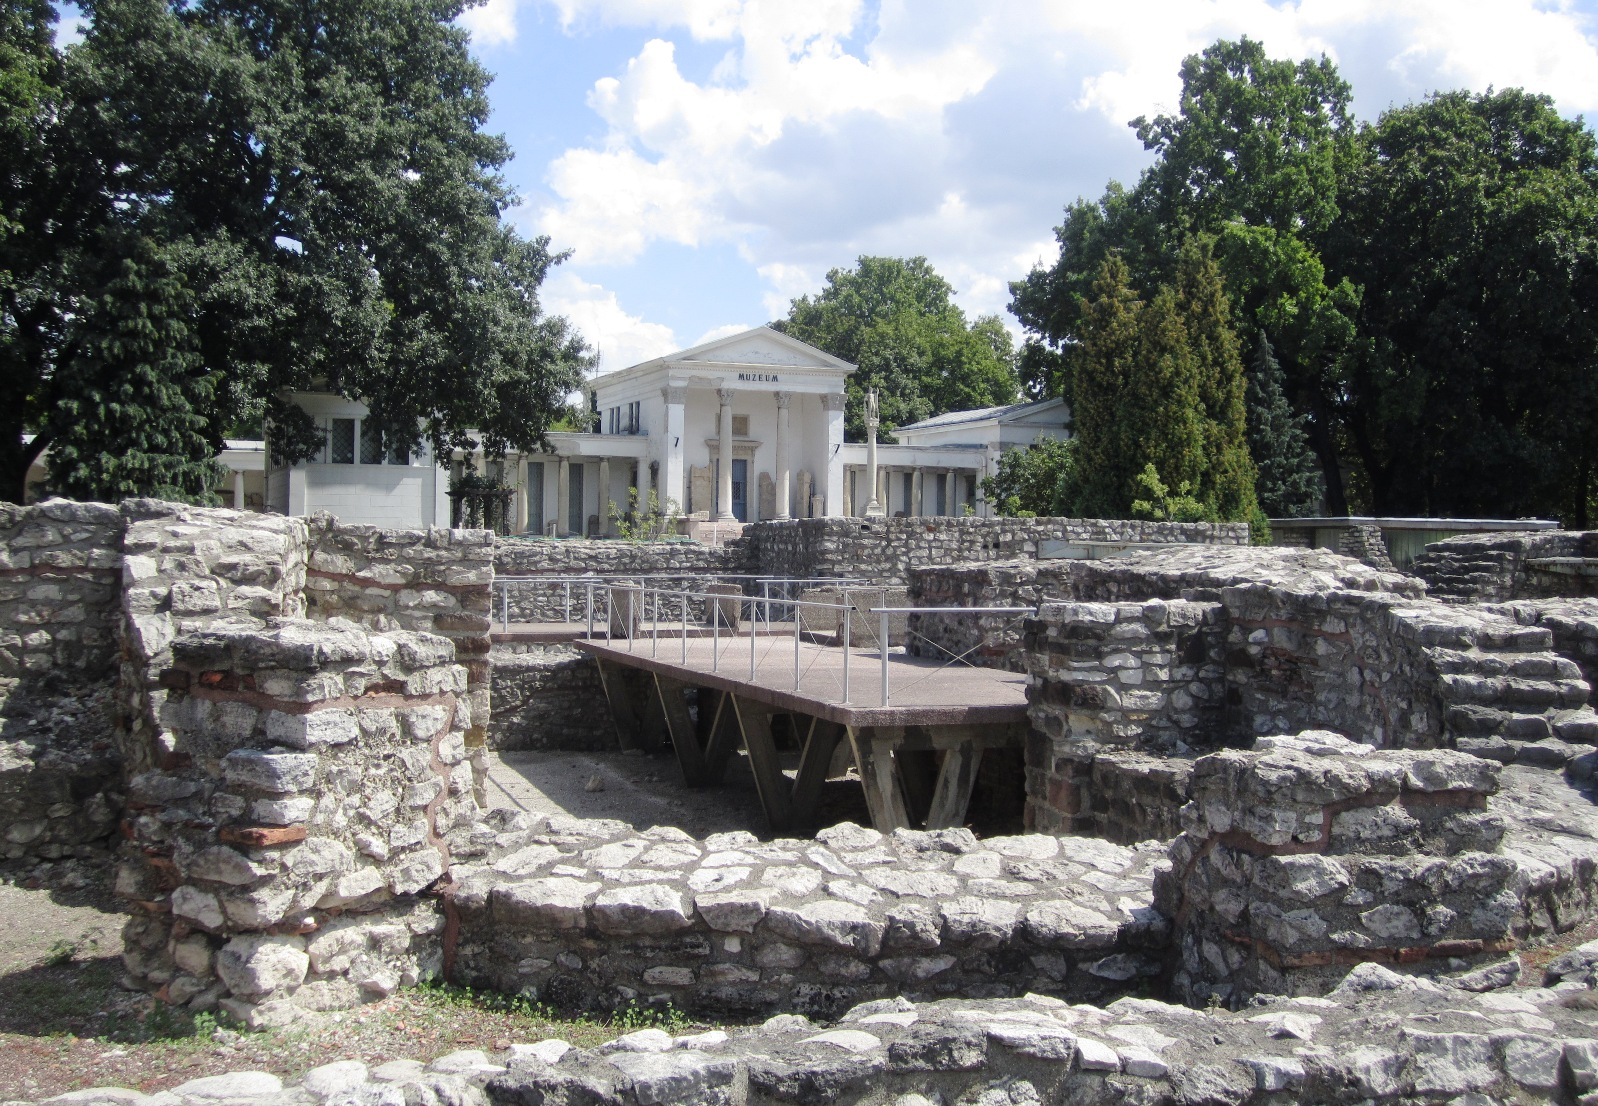
\includegraphics[width=1.0\linewidth]{03/aquincum}
	}
\end{wrapfigure}

\paragraph{Aquincum}
Budapest területén belül is több helyen találhatunk római emlékeket - a legismerebb, legjobban fennmaradt a mai Óbuda területén található Aquincum. Az egykori római települést és katonai tábort 89 körül alapították, virágkora a 2-3. századra esett, de egészen a 4. századik létezett. A főváros területén talált római emlékek legjelentősebb (és természetesen mozdítható) darabjait az Aquincumi Múzeumban tekinthetjük meg (itt találhatóak a római kori polgárváros maradványai is). 

\paragraph{Gorsium}
Gorsium hazánk egyik legjelentősebb római kori települése - a mai Tác község területén (Székesfehérvártól kb 15 km-re) található. A város már az 1. században létezett, több támadást is túlélt, végül hanyatlása a 4. században kezdődött meg, de az eredetileg 400 hektáros területén még évszázadokig laktak. A mai romterület, azaz a Gorsium Régészeti Park, nagyjából 200 hektáros, bejárása közel két órát vesz igénybe - a romok között palota, ókeresztény bazilika, közfürdő, hivatalos épületek, lakóházak és laktanya maradványai láthatóak. 

\paragraph{Brigetio}
Talán kévésbé ismert Brigetio neve - a mai Szőny (Komárom) területén a római időkben jelentős katonai tábor és polgárváros volt. Az ásatások során előkerült téglák, bronz pénzérmék, ékszerek és edények a komáromi Klapka György Múzeumban (a kőfaragványok az Igmándi erődben) és a tatai Kuny Domokos Múzeumban tekinthetőek meg. A dunai gátépítés közben azoban arra is fény derült, hogy a terület már a római időkben is fontos fürdőváros volt - hatalmas, mintegy 800 négyzetméteres fürdőkomplexum, valamint csatornázott, padlófűtéses házak romjait sikerült feltárni.

\begin{wrapfigure}{r}{0.45\textwidth}
	\tcbox[colback=darkgray!85!black,
	left=0mm,right=0mm,top=0mm,bottom=0mm,boxsep=1mm,toptitle=0.5mm,bottomtitle=0.5mm,
	title=\centering{Savaria}]{
		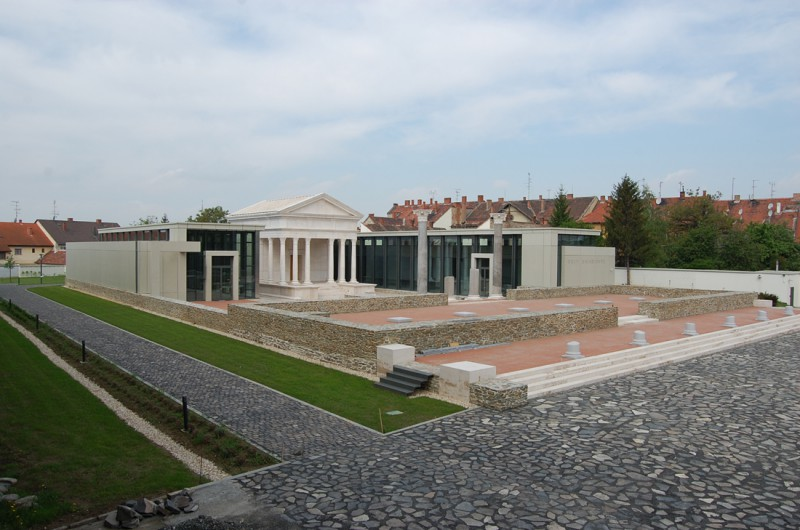
\includegraphics[width=1.0\linewidth]{03/savaria}
	}
\end{wrapfigure}

\paragraph{Savaria}
Savaria Szombathely római kori neve - ez a város volt a Borostyánút egyik állomása, a 2. századtól Felső-Pannonia vallási központja, később tartományi székhely. A római emlékek egy része a Járdányi Paulovics István Romkertben látható - itt az 1937-es ásatások során tártak fel jelentős épületcsoportokat: egy egykori palotát, és annak pazar mozaikpadlóját, római kori fürdőházat és Mercurius-szentély alapfalait is.


\clearpage

\section{A római kori festészet alapvető jellemzői}

\tcbox[left=0mm,right=0mm,top=0mm,bottom=0mm,boxsep=0mm,
toptitle=0.5mm,bottomtitle=0.5mm,title=\centering{A tétel adatai}]{%
\begin{tabular}{| p{0.25\textwidth} | p{0.7\textwidth} |}
	\hline
	Tétel teljes címe 
	&
	Egy konkrét alkotáson keresztül ismertesse a római kori festészet alapvető jellemzőit! Beszéljen a Pompeii-ben feltárt falfestmények alapján a négy meghatározó festészeti stílusáról! Mi az enkausztika?
	\\ \hline
	
\end{tabular}}

\subsection*{Pompeii festményeinek 4 stílusa}

A falfestés stílusai Pompejiben - a római festészet legszebb emlékeit Pompejiben és
Herculaneumban láthatjuk - a Vezúv Kr. u. 79-ben betemette a városokat, majd 1748-ban
fedezték fel - a falfestmények négy különböző stílust képviselnek, külön és keveredve is
előfordulnak.

\subsubsection{Összefoglalás}

\begin{enumerate}
	\item  \textbf{Inkrusztációs stílus} - a falfestmények berakásokat utánoznak, márványból készült
	falburkolat hatását keltik.
	
	\item  \textbf{Architektonikus stílus} - építészeti elemek ábrázolásával látszólag bővítették a teret. 
	
	\item \textbf{ Ornamentális stílus} - mitológia jeleneteket feldolgozó dekoratív stílus, keretezet
	táblakép illúzióját keltve.
	
	\item\textbf{ Illuzionisztikus stílus} - tájképek, csendéletek, épületek valószerűen ábrázolt látszatát
	festették - a mélység irányába futó vonalak párhuzamosak (axonometria) - használták a
	színperspektívát.
\end{enumerate} 

\tcbox[colback=darkgray!85!black,
left=0mm,right=0mm,top=0mm,bottom=0mm,boxsep=1mm,toptitle=0.5mm,bottomtitle=0.5mm,
title=\centering{Pompeii 4 stílusa}]{
	\includegraphics[width=1.0\linewidth]{03/"Pompeji 4 stilusa"}
}


\subsubsection{A falfestészet}

A pompeji ház minden szobáját kifestették, kivéve a gazdasági rendeltetésű helyiségeket
(éléskamra, konyha), valamint a rabszolgák lakószobáit. A falfestészet korántsem volt
állandó jellegű a város egész fennállásának folyamán: változott a megrendelők társadalmi
helyzete, változott az ízlés és ezzel együtt a festészet stílusa is változásokon ment
keresztül. A festők általában a freskó-technikát alkalmazták: a friss vakolatra festettek.
Az alapot előzőleg különleges eljárásokkal megdolgozták, hogy egy ideig friss maradjon,
s ne kezdjen száradni már a képfestés közben. A pompeji falfestmények frissen csillogó
színei részben az alap előzetes preparálásának tulajdoníthatók, részben azonban annak is,
hogy a festékek kitűnő minőségűek; a jó festékkeverés nemzedékek kitartó
fáradozásainak és kísérletezéseinek volt az eredménye.


Pompejiben több szépmíves műhely vagy „iskola” működött, melyek mindegyike
kialakította a maga külön művészi szabályait s tagjaik szigorúan ragaszkodtak ezekhez. A
művészi önállóság csupán abban nyilvánulhatott meg, hogy a művész a saját
egyéniségének megfelelően kombinálta és fejlesztette a hagyományos motívumokat. 
Pompeji persze nem volt hangadó centrum; a Rómában uralkodó áramlatokat követte,
Róma pedig a Görögországból és a hellénisztikus Keletről származó irányzatokat. A
pompeji falfestészetben négy stílust különböztetünk meg.

\subsubsection{Inkrusztációs stílus}

Az első stílus az „inkrusztációs stílus” nevet kapta. Lényege abban áll, hogy a falak
vakolatát márványszerűen festették ki, s ily módon a falak azt a benyomást keltik a
szemlélőben, mintha márványlapokból lennének összeillesztve. A falfelületet először
több mezőre osztották, melyeket különféle módokon lehetett kialakítani; majd az egyes
mezőket tarka színekkel bemázolták, s márvány-ereket utánzó vonalakkal hálózták be.
Ennek a stílusnak jó példáját láthatjuk Sallustius házának tablinumában.


A faltő végig sárga, fölötte fekete márványtáblákat utánzó széles sáv húzódik, majd több
sorban elhelyezett keskeny, különböző színű (sárga, zöld, lila) téglalapok következtek. A
festőn kívül még stukkókészítő mester is közreműködött a ház díszítésében. A fal felső
részén stukkóból formált párkányfogazat vonul végig, fölötte ismét színes „márványtáblák” sorai helyezkednek el, majd újra párkányzat következik. Ily módon a
falnak mintegy kétharmadát díszítések borítják.
Ennek a stílusnak teljes-kibontakozását főleg Délos szigetén és a kisázsiai Priéné
városban épült hellénisztikus házak falain figyelhetjük meg. Itáliai változata - melyet
éppen Pompejiben ismerhetünk meg legjobban - kiváltképpen a tisztán architektonikus
részleteket kedvelte: a fal függőleges voltát kihangsúlyozó oszlopokat és pilléreket.
Ezeket elsősorban ajtók, ablakok, fülkék keretezésére alkalmazták, valamint a fal felső
részén, az első és a második párkányzat között. Általában véve ez a stílus kissé merev.
Súlyossága idővel fárasztónak hat, s a fal unalmasnak tűnik.

\subsubsection{Architektonikus stílus}

A második stílus (i. e. II. század vége) elhagyta a stukkó-párkányzatokat, és az első
stílusnak csupán a festészeti elemeit alkalmazta. Tisztára architektonikus festészetnek
lehet nevezni. Az első stílus „megszilárdította” a falat, korláttá varázsolta, mely a
helyiséget elválasztotta a külvilágtól; a második stílus azonban eltávolította ezt a korlátot.

Az oszlopok, féloszlopok és pillérek most már nem csupán az ajtókat keretezték be, s
nemcsak a fal felső részének díszítésére szolgáltak; a művész az egész falfelületet
befestette velük a faltőtől - sőt néha a padlótól - egészen a mennyezetig.
Az arányok gondos mérlegelése és az árnyékok művészi elosztása folytán az igazi fal
eltűnt, s mint a színpadi dekorációknál, elrejtőzött a művész alkotta látszatvalóság
mögött. A festő a perspektíva eszközeivel a térbeli mélység illúzióját varázsolja a néző
szeme elé. A második stílus további fejlődése folyamán a falon monumentális épületek
jelennek meg térbeli egymásmögöttiségben elrendezve: a szemlélőben elenyészik a fal
határoló, korlátozó jellegének érzete. A fal közepére - az épületek közé - rendszerint zárt ajtót festett a művész. A második stílus utolsó periódusában ez az ajtó „megnyílt”, s a szemlélő rajta „kitekintve” fákat, embereket, állatokat - tájakat és mitológiai jeleneteket
láthatott.

A második stílus két különböző elemet egyesített: az architektonikus perspektívát és a
monumentális falfestészetet, melynek az előbbi keretül szolgált. E stílus sikerének titka
részint a faldekorációk gondolati egyszerűségében és tisztaságában rejlik, részint pedig
abban, hogy a művészek pompás architektonikus képeiknek meg tudták adni azt a 
perspektivikus mélységet, mely gyakran csalódásig híven utánozza a valóságot. Ezek az
architektúrák nemcsak a falakat „szüntették meg”, hanem magát a helyiséget is - olyan
kilátóponttá varázsolták, ahonnan gyönyörködni lehetett büszke paloták szépségében és a
mögöttük elterülő táj végtelenbe nyúló messzeségében. Ennek a stílusnak Kis-ázsia
hellénisztikus központjaiban volt a hazája; bajosan lehetett volna még egy ilyen festészeti
stílust találni, amely ennyire illett volna a római uralom terjeszkedési korához.

\subsubsection{Ornamentális stílus}

A harmadik stílus bizonyos értelemben tiltakozást fejezett ki a második ellen. Az utóbbi
stílus - mint mondottuk - „eltűnteti” a falakat: a térbeli mélység illúzióját keltő
épületekkel festi tele őket, melyek mögött még tájak és emberek láthatók. Ezzel szemben
a harmadik stílus sohasem téveszti szem elől, hogy a fal mindenek előtt sík felület: tehát
nem „töri át” sehol, s nem törekszik térbeli, perspektivikus hatásokra. A harmadik stílus
tökéletes példáját láthatjuk a „Százéves jubileum házában”, ahol a fő mező fekete
hátterén mintegy elenyészve apró fehér figurák állnak. Ennek a stílusnak a dekorációi
faliszőnyeget utánoznak.
Pompejibe természetesen voltak igazi faliszőnyegek is, de egy sem maradt meg; csak a
falba vert szögek és a kampók jelzik egykori helyüket. A művész egész képsorozatokat
ábrázolt faliszőnyeg-utánzatán. De hiába keresnénk köztük a római történelemből vagy a
helyi krónikából vett jeleneteket viszont majdnem az egész görög mitológiát láthatjuk
rajtuk, főleg szerelmi történeteket, melyek Ovidius mitológiai költészetének szellemét
sugározzák. 

\subsubsection{ Illuzionisztikus stílus}

A negyedik stílus korai formájának kell tekintenünk azt a kísérletet, amely a „szőnyegelv” és a perspektíva összeegyeztetésére törekedett. Ez persze megvalósíthatatlan, mert a
perspektíva „kitárja”, a „szőnyeg” ellenben „bezárja” a falat. Ennek a próbálkozásnak
egyik példáját láthatjuk Lucretius Fronto házában. A faltő helyett csupán keskeny sáv fut
végig a padlózat fölött; a fal öt mezőre van tagolva; a középső mező sötétpiros „szőnyeg”, rajta Dionysost és Ariadnét ábrázoló kép; ettől jobbra és balra egy-egy fekete „szőnyeg”, arany kandeláberekkel és kis tájképekkel díszítve.
A negyedik és az ötödik sávban architektonikus motívumok szerepelnek: alul nagy ablak
oromtetővel; fölötte - a perspektivikus ábrázolás halvány visszfényeként - egy kerek
épület ión oszlopai, melyek túlságosan vékonyak ahhoz, hogy valóságérzetet
kelthessenek; a körbefutó virágfüzérek még csak jobban kihangsúlyozzák az
architektonikus motívum valószerűtlenségét. Éppen ilyen fantasztikusak a felső fríz
épületei, bár közöttük valóságosan létező típusokat is lehet látni: a középen egy
háromajtós bazilikát, s mindegyik oldalon egy-egy ctediculát, felettük fedélszerkezettel.
Ám a bazilika közepét kis csendélet foglalja el, fölötte pedig háromlábú üst (tripus)
látható - mintha a művész figyelmeztetni akarná a nézőt, hogy kompozícióját
semmiképpen ne tekintse egy valóságos épület ábrázolásának.

A harmadik stílus - melynek finomságát Pompejiben meg sem közelíti a többi - túlságosan „akadémikus” volt ahhoz, hogy nagy sikerre számíthatott volna. S ha a
köztársaság korának megrázkódtatásaitól, a császárság korának üldöztetéseitől kimerült 
régi arisztokrácia a házaiba vonult vissza, hogy legalább otthon élvezzen ideig-óráig
nyugalmat, biztonságot és békességet - az Imperium támogatását élvező kereskedelem és
ipar képviselői még otthonukban sem óhajtottak elszakadni a világtól; házi kényelmet
akartak, de nem kívántak lemondani a világ csábító messzeségeiről.
A „szőnyeg-stílus” és a perspektíva összehangolására irányuló kísérlet ebből a
szemléletből, ebből a lelki beállítottságból fakadt. A város pusztulása természetesen véget
vetett a pompeji falfestészet további fejlődésének. Itt-ott meg lehet figyelni újabb stílusok
csíráit, de ezek már nem bontakozhattak ki.


\subsection*{A misztériumok villája}

\tcbox[colback=darkgray!85!black,
left=0mm,right=0mm,top=0mm,bottom=0mm,boxsep=1mm,toptitle=0.5mm,bottomtitle=0.5mm,
title=\centering{A misztériumok villájának freskója}]{
	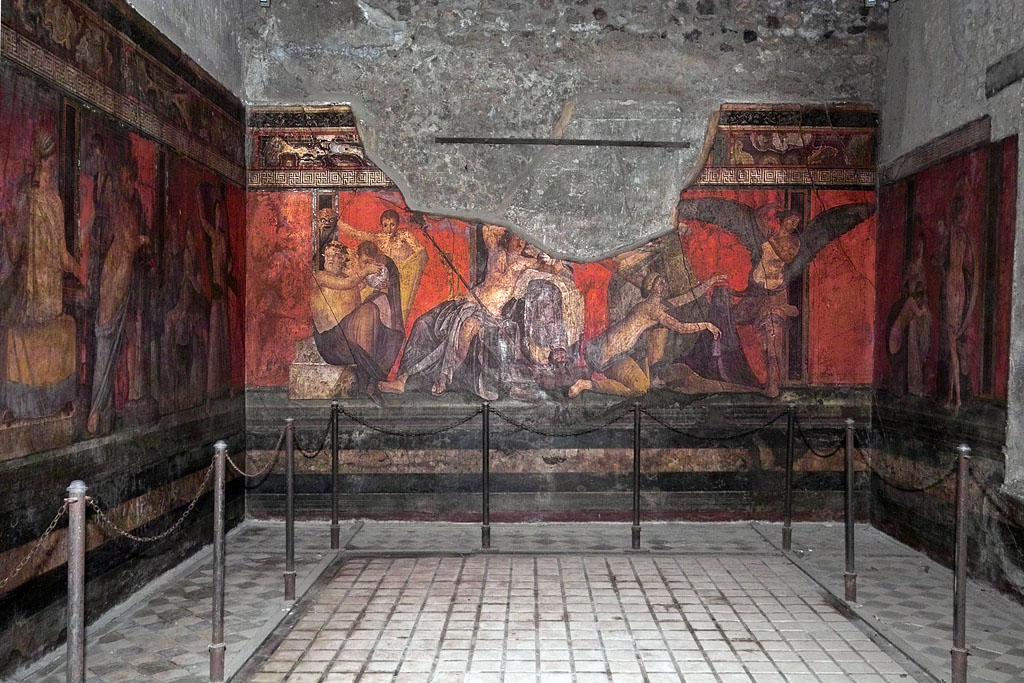
\includegraphics[width=1.0\linewidth]{03/miszteriumok_villaja}
}

A Misztériumok villája Kr. e. 2. században épült, majd az 1. század során újjáépítették. Egyike a több mint 100 római villának, amelyeket a Vezúv környékén feltártak. A Herculaneumi-kaputól nem messze található a Via dei Sepolcri mentén.

Lakóhelyiségeit a második pompeii korszak (architektonikus stílus) stílusjegyeit viselő falfestmények díszítik. Az egyik legérdekesebb freskó egy misztériumjátékot (rituálét) ábrázol, amely során egy fiatal nőt beavatnak a házasság misztériumába (innen származik az épület elnevezése is). Ugyanakkor számos harmadik pompeii korszakbeli falfestmény is található, ezek főleg egyiptomi motívumokat ábrázolnak.

\paragraph{Architektonikus stílus jellemzői}
\begin{compactitem}
	\item Párkányzatok, oszlopok, építészeti elemek tagolják, keretezik a képeket.
	
	\item A képek a tér folytatásaként jelennek meg, kitágítják a teret. Olyan hatást keltenek, mintha a jelenet a szoba folytatásában, a szemlélő körül játszódnának.
\end{compactitem}

\subsection*{Enkausztika}

\subsubsection{Története}
Az enkausztika az egyik legrégebbi festőtechnika. Egyben a legidőtállóbb is.
Magát a méhviaszt, mint festék-kötőanyagot i.e. 3000 óta ismerik.
Egyiptomból az i.e. 2. századból maradtak fenn fatáblára enkausztikával festett portrék, frissességükből mit sem veszített, ép állapotban. Ezek a legrégibb fenn maradt emlékei e technikának, melynek eredete még régebbre nyúlik vissza Görögországban. Kezdetben csak ipari célokra alkalmazták a technikát, hajók festésére.

Az enkausztika lényege az, hogy \textbf{melegen folyós viaszfestékkel festenek}.
Mivel csak melegen alakítható a viaszfesték, nehéz vele dolgozni. Maga az enkausztika szó is melegen való festésre utal.

A viasz a mézgyártás mellékterméke és az ókortól fogva mindig nagy mennyiségben állt rendelkezésre. Plinius történeti írásai szerint a görögök igen régi időktől fogva alkalmazták ezt a technikát. Írott források falfestészetben is megemlítik alkalmazását. Fennmaradt néhány viaszfestő művész neve is, mint pl. Pausias, aki virágcsokrokat és emberalakokat festett magas színvonalon, amiért nagy hírnévre tett szert a maga korában.

Az enkausztikával készült festményeket gyönyörű mély fény, egymásba lágyan olvadó, tüzes színek jellemzik.

Valójában még a mai napig sem sikerült kideríteni, hogy az ókori görögök hogyan készítették el a viaszfestéket és miként dolgoztak vele. A fennmaradt írásos adatok arról számolnak be, hogy ún. punviaszt használtak hozzá. Ezt tengervízben szóda hozzáadásával felforralták, majd a holdfény hatásának tették ki.

Bonyolult eljárás során készültek el a festék pigmenteket tartalmazó színes viaszpaszták, melyeket alapozatlan fatáblára vittek fel egy hosszú nyelű fémeszközzel és meleg állapotában simították el. Kis kályhákkal melegítették mind a fémeszközöket, mind a viaszt. Ilyen fémeszközöket régészeti feltárások során is találtak.

Később, az ókort követően, feledésbe merült e tartós technika és csak a 19. századtól kezdték újra felfedezni.

\subsubsection{A technika jellemzői}

\paragraph{Kötőanyag}
Az enkausztika technikánál a méhviasz a kötőanyag. Kizárólag melegítve használható festésre, amikor folyóssá válik.

\paragraph{Hordozó}
Az enkausztika festményalapjai lehetnek: fatáblák, farostlemez, fémlap, papír, vászon. Egykor kőre, márványra, agyagtáblára is készültek festmények.

\paragraph{Alapozás}
Az ókorban alapozott és alapozatlan felületekre festettek ezzel a technikával. Manapság sem szükséges alapozás a farostlemezekre, de a rajz - és akvarell papírokra sem. Ha mégis alapozzák, viasszappant keverenek az alapozószerbe és vékonyan kenik fel. Vásznakra is így készül alapozás.

\paragraph{Pigment}
Minden fényálló pigment alkalmas ehhez a technikához, finoman őrölve. Csak azokról a pigmentekről kell lemondani, amelyek nem viselik el a 80 C fok fölötti hőmérsékletet (a viasz olvadása miatt). Házilag való elkészítésük nagy tapasztalatot igényel.

\paragraph{A technika alapanyagjának nehézségei}
A 20. században a legelső enkausztika festéket gyártó gyár csődbe ment, a kereslet csekély volta miatt. Igen kevés művész alkalmazza ma is ezt a technikát és kevés cég gyárt hozzá festékeket, sokszor nem is az eredeti technikának megfelelően. Ilyenek pl. a viaszfestékkréták. Bár házilag nagyon nehéz előállítani az enkausztika festéket, azok a művészek, akik használják, mégis maguk készítik el.

Ez a már megszűnt, egykori cég kockák formájában árulta a viszfestékeket és elektromosan fűthető palettákat kínált hozzájuk. Ecsettel festettek, és ha félretették az ecsetet, rögtön megdermedt benne a viaszfesték, amikor kihűlt, de felmelegítve újra folyóssá vált. A festőfelületet is melegítették. Az ecseteket lakkbenzinnel mosták ki használat után.

Maga a viasz víztaszító és igen ellenálló tulajdonságú. Gyártása során kifehérítik. Olvadáspontja 63-65 C fok körüli.

Festék készítésekor a pigmenteket összeolvasztják a méhviasszal. A festék eloszlatása a festőfelületen is hőközléssel történik.

\paragraph{Eszközök}
Elektromosan fűthető palettákat használnak a viaszfesték olvadt, folyékony állapotban tartásához. Írópulthoz hasonló állványra kerülnek a hordozók. Hősugárzókkal történik a festőfelület melegítése. Festéshez a sörteecsetek és a spatulák a legmegfelelőbbek.

A fűtött spatulák manapság gyengeárammal működnek, így teljesen veszélytelenek. A spatulák különböző formájú és méretű spatulapapucsokkal egészíthetők ki. A kézi hősugárzókat manapság infravörös lámpákkal is helyettesítik.

A festőfelületet elölről vagy hátulról melegítik. A szilárd, kemény enkausztika festékek kb. 70 fokon válnak folyékonnyá és festhető állagúvá.

A mai enkausztik technika az elektromosan fűthető eszközök segítségével sokkal könnyebbé vált, mint az ókorban.

\paragraph{Folyamat}
A festmények vázlatai készülhetnek szénnel, krétával, ceruzával, akvarellel stb. a hordozókra. Erre kerülnek azután a viaszfestékek.

Az elkészült képet, ha megdermedt a kihűlt viasz, gyapjú ronggyal utólag csillogóvá polírozhatjuk.

A technika előnyei: a viaszfestmény nem sárgul, nem repedezik, nem zsugorodik, ellenáll a nedvességnek, időtálló évezredeken keresztül, ahogy a fennmaradt képek is bizonyítják. Gyakorlatilag örökéletű. Egyetlen veszély fenyegeti: a hőhatás, amitől megolvadhat vagy eléghet. Sajnos a történelem viharaiban, háborúk és tűzvészek során ennek estek áldozatul az enkausztika festmények.

A festést, ha abbahagyjuk, megdermed a festék, amit akár évek múlva is folytathatunk, újra felmelegítve.